\ifx\wholebook\relax\else

% --------------------------------------------
% Lulu:

    \documentclass[a4paper,12pt,twoside]{../includes/ThesisStyle}

	\usepackage[T1]{fontenc} %%%key to get copy and paste for the code!
%\usepackage[utf8]{inputenc} %%% to support copy and paste with accents for frnehc stuff
\usepackage{times}
\usepackage{ifthen}
\usepackage{xspace}
\usepackage{alltt}
\usepackage{latexsym}
\usepackage{url}            
\usepackage{amssymb}
\usepackage{amsfonts}
\usepackage{amsmath}
\usepackage{stmaryrd}
\usepackage{enumerate}
\usepackage{cite}
%\usepackage[pdftex,colorlinks=true,pdfstartview=FitV,linkcolor=blue,citecolor=blue,urlcolor=blue]{hyperref}
\usepackage{xspace}
%\usepackage{graphicx}
\usepackage{subfigure}
\usepackage[scaled=0.85]{helvet}
        
        
\newcommand{\sepe}{\mbox{>>}}
\newcommand{\pack}[1]{\emph{#1}}
\newcommand{\ozo}{\textsc{oZone}\xspace}
\newcommand\currentissues{\par\smallskip\textbf{Current Issues -- }}

\newboolean{showcomments}
\setboolean{showcomments}{true}
\ifthenelse{\boolean{showcomments}}
  {\newcommand{\bnote}[2]{
	\fbox{\bfseries\sffamily\scriptsize#1}
    {\sf\small$\blacktriangleright$\textit{#2}$\blacktriangleleft$}
    % \marginpar{\fbox{\bfseries\sffamily#1}}
   }
   \newcommand{\cvsversion}{\emph{\scriptsize$-$Id: macros.tex,v 1.1.1.1 2007/02/28 13:43:36 bergel Exp $-$}}
  }
  {\newcommand{\bnote}[2]{}
   \newcommand{\cvsversion}{}
  } 


\newcommand{\here}{\bnote{***}{CONTINUE HERE}}
\newcommand{\nb}[1]{\bnote{NB}{#1}}
\newcommand{\fix}[1]{\bnote{FIX}{#1}}
%%%% add your own macros 

\newcommand{\sd}[1]{\bnote{Stef}{#1}}
\newcommand{\ja}[1]{\bnote{Jannik}{#1}}
\newcommand{\na}[1]{\bnote{Nico}{#1}}
%%% 


\newcommand{\figref}[1]{Figure~\ref{fig:#1}}
\newcommand{\figlabel}[1]{\label{fig:#1}}
\newcommand{\tabref}[1]{Table~\ref{tab:#1}}
\newcommand{\layout}[1]{#1}
\newcommand{\commented}[1]{}
\newcommand{\secref}[1]{Section \ref{sec:#1}}
\newcommand{\seclabel}[1]{\label{sec:#1}}

%\newcommand{\ct}[1]{\textsf{#1}}
\newcommand{\stCode}[1]{\textsf{#1}}
\newcommand{\stMethod}[1]{\textsf{#1}}
\newcommand{\sep}{\texttt{>>}\xspace}
\newcommand{\stAssoc}{\texttt{->}\xspace}

\newcommand{\stBar}{$\mid$}
\newcommand{\stSelector}{$\gg$}
\newcommand{\ret}{\^{}}
\newcommand{\msup}{$>$}
%\newcommand{\ret}{$\uparrow$\xspace}

\newcommand{\myparagraph}[1]{\noindent\textbf{#1.}}
\newcommand{\eg}{\emph{e.g.,}\xspace}
\newcommand{\ie}{\emph{i.e.,}\xspace}
\newcommand{\ct}[1]{{\textsf{#1}}\xspace}


\newenvironment{code}
    {\begin{alltt}\sffamily}
    {\end{alltt}\normalsize}

\newcommand{\defaultScale}{0.55}
\newcommand{\pic}[3]{
   \begin{figure}[h]
   \begin{center}
   \includegraphics[scale=\defaultScale]{#1}
   \caption{#2}
   \label{#3}
   \end{center}
   \end{figure}
}

\newcommand{\twocolumnpic}[3]{
   \begin{figure*}[!ht]
   \begin{center}
   \includegraphics[scale=\defaultScale]{#1}
   \caption{#2}
   \label{#3}
   \end{center}
   \end{figure*}}

\newcommand{\infe}{$<$}
\newcommand{\supe}{$\rightarrow$\xspace}
\newcommand{\di}{$\gg$\xspace}
\newcommand{\adhoc}{\textit{ad-hoc}\xspace}

\usepackage{url}            
\makeatletter
\def\url@leostyle{%
  \@ifundefined{selectfont}{\def\UrlFont{\sf}}{\def\UrlFont{\small\sffamily}}}
\makeatother
% Now actually use the newly defined style.
\urlstyle{leo}



	\usepackage{amsmath,amssymb}             % AMS Math
% \usepackage[french]{babel}
\usepackage[latin1]{inputenc}
\usepackage[T1]{fontenc}
\usepackage[left=1.5in,right=1.3in,top=1.1in,bottom=1.1in,includefoot,includehead,headheight=13.6pt]{geometry}
\renewcommand{\baselinestretch}{1.05}

\usepackage{multicol}

% Table of contents for each chapter

\usepackage[nottoc, notlof, notlot]{tocbibind}
\usepackage{minitoc}
\setcounter{minitocdepth}{1}
\mtcindent=15pt
% Use \minitoc where to put a table of contents

\usepackage{enumitem}

\usepackage{aecompl}

% Glossary / list of abbreviations

%\usepackage[intoc]{nomencl}
%\renewcommand{\nomname}{List of Abbreviations}
%
%\makenomenclature

% My pdf code

\usepackage[pdftex]{graphicx}
\usepackage[a4paper,pagebackref,hyperindex=true]{hyperref}

\usepackage{pgfplotstable,booktabs,colortbl}
\pgfplotsset{compat=1.8}

% Links in pdf
\usepackage{color}
\definecolor{linkcol}{rgb}{0,0,0.4} 
\definecolor{citecol}{rgb}{0.5,0,0} 

% Change this to change the informations included in the pdf file

% See hyperref documentation for information on those parameters

\hypersetup
{
bookmarksopen=true,
pdftitle="Sista: a Metacircular Architecture for Runtime Optimisation Persistence",
pdfauthor="Clement BERA", 
pdfsubject="Thesis", %subject of the document
%pdftoolbar=false, % toolbar hidden
pdfmenubar=true, %menubar shown
pdfhighlight=/O, %effect of clicking on a link
colorlinks=true, %couleurs sur les liens hypertextes
pdfpagemode=None, %aucun mode de page
pdfpagelayout=SinglePage, %ouverture en simple page
pdffitwindow=true, %pages ouvertes entierement dans toute la fenetre
linkcolor=linkcol, %couleur des liens hypertextes internes
citecolor=citecol, %couleur des liens pour les citations
urlcolor=linkcol %couleur des liens pour les url
}

% definitions.
% -------------------

\setcounter{secnumdepth}{3}
\setcounter{tocdepth}{1}

% Some useful commands and shortcut for maths:  partial derivative and stuff

\newcommand{\pd}[2]{\frac{\partial #1}{\partial #2}}
\def\abs{\operatorname{abs}}
\def\argmax{\operatornamewithlimits{arg\,max}}
\def\argmin{\operatornamewithlimits{arg\,min}}
\def\diag{\operatorname{Diag}}
\newcommand{\eqRef}[1]{(\ref{#1})}

\usepackage{rotating}                    % Sideways of figures & tables
%\usepackage{bibunits}
%\usepackage[sectionbib]{chapterbib}          % Cross-reference package (Natural BiB)
%\usepackage{natbib}                  % Put References at the end of each chapter
                                         % Do not put 'sectionbib' option here.
                                         % Sectionbib option in 'natbib' will do.
\usepackage{fancyhdr}                    % Fancy Header and Footer

% \usepackage{txfonts}                     % Public Times New Roman text & math font
  
%%% Fancy Header %%%%%%%%%%%%%%%%%%%%%%%%%%%%%%%%%%%%%%%%%%%%%%%%%%%%%%%%%%%%%%%%%%
% Fancy Header Style Options

\pagestyle{fancy}                       % Sets fancy header and footer
\fancyfoot{}                            % Delete current footer settings

%\renewcommand{\chaptermark}[1]{         % Lower Case Chapter marker style
%  \markboth{\chaptername\ \thechapter.\ #1}}{}} %

%\renewcommand{\sectionmark}[1]{         % Lower case Section marker style
%  \markright{\thesection.\ #1}}         %

\fancyhead[LE,RO]{\bfseries\thepage}    % Page number (boldface) in left on even
% pages and right on odd pages
\fancyhead[RE]{\bfseries\nouppercase{\leftmark}}      % Chapter in the right on even pages
\fancyhead[LO]{\bfseries\nouppercase{\rightmark}}     % Section in the left on odd pages

\let\headruleORIG\headrule
\renewcommand{\headrule}{\color{black} \headruleORIG}
\renewcommand{\headrulewidth}{1.0pt}
\usepackage{colortbl}
\arrayrulecolor{black}

\fancypagestyle{plain}{
  \fancyhead{}
  \fancyfoot{}
  \renewcommand{\headrulewidth}{0pt}
}

\usepackage{algorithm}
\usepackage[noend]{algorithmic}

%%% Clear Header %%%%%%%%%%%%%%%%%%%%%%%%%%%%%%%%%%%%%%%%%%%%%%%%%%%%%%%%%%%%%%%%%%
% Clear Header Style on the Last Empty Odd pages
\makeatletter

\def\cleardoublepage{\clearpage\if@twoside \ifodd\c@page\else%
  \hbox{}%
  \thispagestyle{empty}%              % Empty header styles
  \newpage%
  \if@twocolumn\hbox{}\newpage\fi\fi\fi}

\makeatother
 
%%%%%%%%%%%%%%%%%%%%%%%%%%%%%%%%%%%%%%%%%%%%%%%%%%%%%%%%%%%%%%%%%%%%%%%%%%%%%%% 
% Prints your review date and 'Draft Version' (From Josullvn, CS, CMU)
\newcommand{\reviewtimetoday}[2]{\special{!userdict begin
    /bop-hook{gsave 20 710 translate 45 rotate 0.8 setgray
      /Times-Roman findfont 12 scalefont setfont 0 0   moveto (#1) show
      0 -12 moveto (#2) show grestore}def end}}
% You can turn on or off this option.
% \reviewtimetoday{\today}{Draft Version}
%%%%%%%%%%%%%%%%%%%%%%%%%%%%%%%%%%%%%%%%%%%%%%%%%%%%%%%%%%%%%%%%%%%%%%%%%%%%%%% 

\newenvironment{maxime}[1]
{
\vspace*{0cm}
\hfill
\begin{minipage}{0.5\textwidth}%
%\rule[0.5ex]{\textwidth}{0.1mm}\\%
\hrulefill $\:$ {\bf #1}\\
%\vspace*{-0.25cm}
\it 
}%
{%

\hrulefill
\vspace*{0.5cm}%
\end{minipage}
}

\let\minitocORIG\minitoc
\renewcommand{\minitoc}{\minitocORIG \vspace{1.5em}}

\usepackage{multirow}
\usepackage{slashbox}

\newenvironment{bulletList}%
{ \begin{list}%
	{$\bullet$}%
	{\setlength{\labelwidth}{25pt}%
	 \setlength{\leftmargin}{30pt}%
	 \setlength{\itemsep}{\parsep}}}%
{ \end{list} }

\newtheorem{definition}{D�finition}
\renewcommand{\epsilon}{\varepsilon}

% centered page environment

\newenvironment{vcenterpage}
{\newpage\vspace*{\fill}\thispagestyle{empty}\renewcommand{\headrulewidth}{0pt}}
{\vspace*{\fill}}



	\graphicspath{{.}{../figures/}}
	\begin{document}
\fi

\chapter{Runtime evolutions}
\label{chap:runtimeEvolution}
\minitoc

%Generic intro
To support the architecture described in the previous chapter, the Pharo runtime had to evolve. We distinguish two kind of evolutions. Some evolutions were required to support the architecture, the Sista runtime could not work without those features. Other evolutions were not mandatory, the Sista architecture could have worked without these features, but each of them were important to improve the overall performance.

%%%%%%%%%%%%%%%%%%%%%%%%%%%%%%%%%%%%%%%%%%%%%%%%%%%%%%%%%%%%%%%%%%%%%%%%%%%%%%%%%%%%%%%%%%%%%%%%%%%%%%%%%%%%%%%%%%%%%%%%%%%%%%%%%%%%
%%%%%%%%%%%%%%%%%%%%%%%%%%%%%%%%%%%%%%%%%%%%%%%%%%%%%%%%%%%%%%%%%%%%%%%%%%%%%%%%%%%%%%%%%%%%%%%%%%%%%%%%%%%%%%%%%%%%%%%%%%%%%%%%%%%%

\section{Required language evolutions}

Five major evolutions were required to have the Sista architecture up and running:
\begin{enumerate}
	\item Cogit was extended to detect hot spots through profiling counters.
	\item The interpreter and Cogit were extended to be able to execute and compile the additional instructions of the extended bytecode set.
	\item Two VM call-backs were added to trigger Scorch when a hot spot is detected or a guard fails.
	\item A new primitive was introduced to provide runtime information in Smalltalk for v-functions having a corresponding n-function generated by Cogit.
	\item The Scorch framework, including the optimiser, the deoptimiser and the dependency manager were introduced.
\end{enumerate}

\subsection{Profiling counters}

To detect hot spots, Cogit was extended to be able to generate profiling counters when generating a n-function. When the execution flow reaches a counter, it increases its value by one. If the counter reaches a threshold, the VM trigger a special call-back to activate Scorch Profiling counters induce overhead, which can be significant enough to be seen in some benchmarks (the overhead is detailed in the validation chapter on a set of benchmarks). To avoid the overhead in optimised code, Cogit was extended to support conditionnal compilation. Based on a bit in a v-function's header, Cogit generates a n-function with or without profiling counters. 

Based on \cite{Arn02}, profiling counters were added on conditional branches, with one counter just before and one counter just after the conditional branch. This strategy allows the VM to provide basic block usage information in addition to the detection of hot spots. Every finite loop requires a branch to stop the loop iteration and most recursive code requires a branch to stop the recursion, so the main cases for which we wanted to detect hot spots for are covered. Each time the execution flow reaches a conditional branch in a n-function, it increases the profiling counter by one, compares the counter value to a threshold and jumps to the hot spot detection routine if the threshold is reached. If the threshold is not reached, the conditional branch is performed. If the branch is not taken, a second counter is incremented by one to provide later basic block usage information.

The main issue we had to deal with when implementing profiling counters is the location of the counters and the access to the counters. Indeed, in our first naive implementation, the counter values were directly inlined in the native code. That was a terrible idea as every write near executable code flushes part of the processor instruction cache, leading to horrible performance. In the end, we changed the logic to allocate a pinned unsigned 32-bits integer array\footnote{A pinned object is an object that can never be moved in memory. For example, the garbage collector cannot move it.} for each n-function requiring counters. The pinned array is on heap, far from executable code, and contains all the counter values. As the array is pinned, the native code can access the array and each of its fields (each counter) through a constant address. This is very nice as the native code can be efficient by using constant addresses and the n-function does not require any metadata~\footnote{References to non pinned objects from n-function normally require metadata to update the reference when the object is moved in memory, typically by the garbage collector.}.

\begin{figure}[h!]
    \begin{center}
        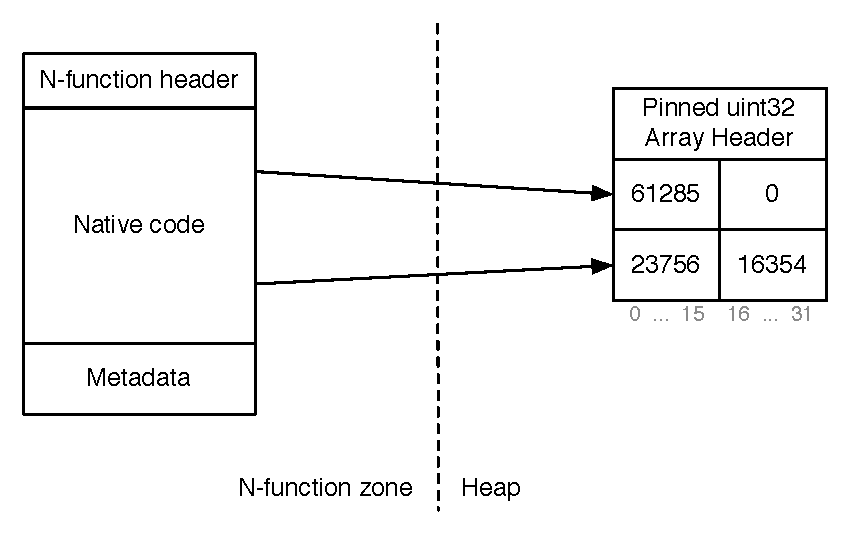
\includegraphics[width=0.8\linewidth]{ProfilingCounters}
        \caption{Non optimised n-function with two profiling counters}
        \label{fig:ProfilingCounters}
    \end{center}
\end{figure}

Figure \ref{fig:ProfilingCounters} shows a n-function with two profiling counters. The n-function is present in the n-function zone, with is readable, writable and executable. The n-function zone is exclusively modified by Cogit. The pinned array is allocated on heap, where all objects are present, which is a readable and writable (but not executable) zone. The n-function is composed of a header, which encodes different properties of the n-function such as its size, the n-function native code and metadata to be able to introspect the n-function. As this n-function requires two counters, an array with two 32 bits wide fields is allocated on heap. Each 32 bits counter field is split in two. The high 16 bits are used for the counter just before the conditional branch, precising how many times the branch has been reached. The low 16 bits are used for the counter just after the branch, precising how many times the branch was not taken. The native code has direct references to the counter addresses. The n-function header has also a reference to the pinned array, not shown on the figure to avoid confusion, which is used to reclaim the pinned array memory when the n-function is garbage collected. In the example, we can see that the first branch is always taken (the counter increased when the branch is not taken is at 0 while the branch has been reached 61285 times).

\subsection{Extended bytecode set}

The Sista architecture required an extended bytecode set to support all the new operations permitted only in optimised v-functions. The new operations were described in one of our IWST paper\cite{Bera14a}. The extended bytecode set design relies on the assumption that only a small number of new instructions are needed for Cogit to produce efficient machine code. Four main kind of instructions were introduced:
\begin{itemize}
\item \textbf{Guards}: Guards are used to ensure an optimisation-time assumption is valid at runtime. If the guard fails at runtime, the dynamic deoptimisation routine is triggered.
\item \textbf{Object unchecked accesses}: Normally variable-sized objects such as arrays or byte arrays require bounds checks to allow a program to access their fields. Unchecked access directly reads the field of an object without any checks. Instructions to access the size of a variable-sized object without any checks are included.
\item \textbf{Unchecked arithmetics}: Arithmetic operations need to check for the operand types to know what arithmetic operation to execute (integer operation, double operation, etc.). Unchecked operations are typed and do not need these check. In addition, unchecked operations do not perform any overflow check.
\item \textbf{Unchecked object allocation and stores}: Normal object allocations do many different things in addition to memory allocation, such as the initialization of all fields to \ct{nil} which is not needed if all fields are set immediately after to other values. Normal stores into objects go through a write barrier to make sure that the store does not break any garbage collector invariant. Such a write barrier can be ignored in specific cases, for example when doing a store in an object that has just been allocated, because it is guaranteed to be in the young object space.
\end{itemize}

As discussed in the previous chapter, optimised v-functions may be interpreted but we made sure that their interpretation is very uncommon. We designed the unsafe operations to be efficient when an optimised n-function is generated to execute the optimised v-function. We did not design the unsafe operations for efficient interpretation. Designing the operations for efficient native code generation is quite different from designing them for efficient interpretation. For efficient native code generation, we encoded the unsafe operations in multiple bytes to be able to provide extra information to Cogit on how to produce good native code for the instruction. This strategy is not very good for the interpreter as it needs additional time to decode the multiple bytes. A good design for efficient interpretation would have been to encode performance critical instructions in a single byte.

%As the optimised methods are represented as bytecodes, they can potentially be executed by the VM interpreter. However, as discussed in the previous chapter, we made sure that it was very uncommon. Improving the performance to speed-up the bytecode interpreter or to speed-up the machine code generated using Cogit are two different tasks that may conflict with one another. We designed the extended bytecode set so the machine code generated by Cogit is as efficient as possible, not really considering the speed of the interpretation of such v-functions.

\subsection{Call-backs}

As the Scorch optimiser and deoptimiser are written in Pharo while the rest of the VM is written in Slang, the VM needs a special way to activate them. 

Pharo has an array of registered objects which can be accessed both from the VM and the language. Among registered objects are specific selectors. One example is the \ct{\#doesNotUnderstand:} selector. When a look-up performed by the VM does not find any method to activate (the selector is not implemented for the given receiver), the VM instead performs a virtual call, using the same receiver, the registered \ct{\#doesNotUnderstand:} selector and reifies the virtual call as an object (which class is also registered) containing the original selector, the arguments and the look-up class in case of a super send. 

We registered two new selectors. One is activated by the VM when a hot spot is detected in a non optimised n-function. The other one is activated when a guard failed in an optimised n-function. A method is implemented in Smalltalk for each selector in the class used for reified stack frames. In our case, these methods activate respectively the Scorch optimiser or the Scorch deoptimiser.

\subsection{Machine code introspection}

%what does the primitive + intro
To extract runtime information from a n-function, we added a new primitive method called \emph{sendAndBranchData}. SendAndBranchData is activated with no arguments and fails if the receiver is not a v-function. If the v-function was compiled by Cogit and therefore has an associated n-function, the primitive answers runtime information present for the function, if the v-fucntion was not compiled, the primitive fails. The runtime information includes types and functions met at each inline cache and the profiling counters values. This information can be then used by Scorch to speculate on types and basic block usage. 

%reading the cache/counter through 
Cogit had an introspection API used for multiple features such as inline cache relinking or debugging. The cache and counter values are read by the implementation of a small extension on top of Cogit's API for introspection. In non optimised n-function, Cogit generates an inline cache for each virtual call~\cite{Deut84a,Holz91a}, relinked at runtime each time a new receiver type is met for the call. The caches can be read using low-level platform-specific code, similar to the code used for relinking. Cogit generates for each profiling counter a call to the hot spot detection Slang routine, used to trigger the hot spot detection routine. This call is annotated with the corresponding virtual instruction pointer, allowing Scorch to know to which conditional branch in the v-function each profiling counters correspond to.

%Result of primitive
The new primitive iterates over the n-function, collecting for each virtual call and each conditionnal branch the virtual instruction pointer as well as respectively type and profiling information. Because the data is collected from Slang, it's not convenient to build complex data structure using multiple different kind of objects (Each object's class internal representation would need to be specifically known by both the VM and the language). To keep things simple, the primitive answers an array of array, each inner array containing the virtual program counter of the instruction, and a list of types and v-functions targetted by the inline cache or the number of times each branch has been taken.

\subsection{Scorch}

In the implementation of the Sista architecture, the bulk of the work was the design and the implementation of the Scorch optimiser. The thesis is centered around the Sista architecture in general and there is no big innovative features in Scorch.

Scorch's optimiser is implemented as a traditionnal optimising compiler. It translates the v-functions to optimise into a single static assignment intermediate representation, represented as a control flow graph. Conditionnal branch and send instructions are annotated with the runtime information provided by Cogit to speculate on what method to inline and on basic block usage.

The optimisation performed are very similar to the ones performed in other optimising JITs such as V8 Crankshaft optimising JIT~\cite{V8}. Scorch starts by speculating on types to inline other functions. Guards are inserted to ensure speculations are valid at runtime. Once inlining is done, Scorch perform multiple standard optimisations such as array-bounds check elimination with the ABCD algorithm~\cite{Bodi00a} or global value numbering. Scorch also attempts to postpone allocation of objects not escaping the optimised v-function from runtime to deoptimisation time (or completely removes the allocation if the object is never required for deoptimisation).

Scorch's back-end generates an optimised v-function from the intermediate representation. The phi instructions from single static assignment are removed, using instead temporary locations assigned multiple times. For each instruction, Scorch determines if the computed value needs to be stored to be reused, and if so, if it can be stored as a spilled value on stack or as a temporary variable. The deoptimisation metadata is attached to the optimised v-function to be able to restore the multiple frames.

Scorch's deoptimiser is much simpler than the optimiser. It reads the deoptimisation metadata for a given program counter in the optimised v-function. The metadata consists of a list of objects to reconstruct, including closures and reified stack frames. The objects are reconstructed by reading constant values in the metadata or reading the optimised stack frame values. Once the objects are reconstructed, execution can resume in the bottom frame restored.

Scorch's dependency manager is also much simpler than the optimiser. It keeps track for each optimised function of the list of selectors it depends on. If a method with one of these selectors is installed, all the optimised functions dependant are discarded. 

%%%%%%%%%%%%%%%%%%%%%%%%%%%%%%%%%%%%%%%%%%%%%%%%%%%%%%%%%%%%%%%%%%%%%%%%%%%%%%%%%%%%%%%%%%%%%%%%%%%%%%%%%%%%%%%%%%%%%%%%%%%%%%%%%%%%
%%%%%%%%%%%%%%%%%%%%%%%%%%%%%%%%%%%%%%%%%%%%%%%%%%%%%%%%%%%%%%%%%%%%%%%%%%%%%%%%%%%%%%%%%%%%%%%%%%%%%%%%%%%%%%%%%%%%%%%%%%%%%%%%%%%%

\section{Optional language evolutions}


Five major evolutions were introduced in the language in addition to the required evolutions to allow Scorch to produce more efficient optimised v-functions:
\begin{enumerate}
	\item A new memory manager for efficient n-function generation.
	\item A new bytecode set to leverage encoding limitations.
	\item A register allocation algorithm in Cogit.
	\item A write barrier feature to be able to mark object as read-only.
	\item A new closure implementation to be able to optimiser closure more efficiently.
\end{enumerate}

\subsection{New memory manager}

%pb with existing representation
The first version of the Sista architecture was built on the existing VM with a minimum number of modifications. One of the main issue met was related to the memory representation of objects. The existing memory manager was designed and implemented before the implementation of Cogit for a pure interpreter VM. The representation of object did not allow Cogit to produce efficient accesses to object fields in native code.

%existing class access
One problem for example was the encoding of the class field in an object. It could be encoded in three different ways:
\begin{itemize}
	\item \emph{Immediate classes:} A very limited subset of classes, included \ct{SmallInteger}, have their instances encoded in the pointer to the object itself. As all objects are aligned in memory for efficient access to their fields, the last few bits (the exact number depends on the alignment) of a pointer to an object are never set. By setting some of these last few bits, the memory manager can encode a class identifier. \ct{SmallInteger} for example are encoded by setting the last bit of the pointer.
	\item \emph{Compact classes:} A limited set of classes, up to 15 classes, had their instances encoding their classes as an index in a 4-bits field in the first word of the object's header. The memory manager had access to an array mapping the indexes to the actual classes.
	\item \emph{Other classes:} All the other instances encoded their class as a pointer to the class object, encoded in an extra pointer-sized field in the header of the object.
\end{itemize}

%existing class access pb in n-functions
In practice, Cogit compiles many type-checks. In non optimised n-functions, type-checks are generated mainly in inline caches. In optimised functions, type-checks are generated for deoptimisation guards. For each type-check, the native code generated needed three paths to find out which one of the three encodings was used for the instance which was type-checked, to finally compare it against the expected type. In addition, as many instances encoded their class as a pointer to the class object while class objects can be moved by the garbage collector in memory, cogit needed to annotate the expected type to correctly update the pointer value during garbage collection. Overall both the generated n-function and the garbage collector were slowed by the memory representation.

%Spur and problem solving
To solve this problem, a new memory manager was implemented and deployed in production~\cite{Mir15a}. The new representation of objects in memory allows the generation of very efficient n-functions. For example, there is now only two ways for an instance to access its class, the class is either immediate or compact. Compact classes indexes are stored in the instances in a 22-bit fields, allowing over four millions different concrete classes. As all references to classes are now through an indirection index, type-checks are not annotated by Cogit when generating the n-function as the garbage collector can ignore them.

%other pbs soled
In addition to allowing the generation of efficient n-functions, other problems non directly related to the thesis were present in the existing memory manager (poor support for large heaps, slow scavenges, etc.) which were solved with the new memory manager.

% pinned objects ??? I don't know if it's worth going into details there.

\subsection{New bytecode set}

The existing Pharo bytecode set had multiple encoding limitations~\cite{Bera14a}. For example, jumps (forward, backward and conditonnal) were able to jump over 1024 bytes at most. Such limitations are very rarely a problem while compiling normal Smalltalk code due to coding convention encouraging developers to write small functions. However, the optimised function produced by Scorch includes many inlined functions and in some case the limitations were a problem. As the bytecode set already needed to be extended to support the new unsafe operations, we designed a complete new bytecode set instead of just adding the new operations to leverage encoding limitations.

\subsection{Register allocation}

To allocate registers, Cogit simulates the stack state during compilation. When reaching an instruction using values on stack, Cogit uses a dynamic template scheme to generate the native instructions. The simulated stack provides information such as which values are constants or already in registers. Based on this information, Cogit picks one of the available template for the instruction, use a linear scan algorithm to allocate registers that do not need to be fixed into specific concrete registers and generate the native instructions.

The existing linear scan algorithm was very naive and limited. It was very efficient because registers are not live across certain instructions that are very common in non optimised code. Specifically, registers cannot be live across these three instructions:
\begin{enumerate}
	\item \emph{virtual calls:} All registers are caller-saved.
	\item \emph{backjumps:} Backjumps are interrupt points.
	\item \emph{Conditionnal branches:} If the branch is on a non-boolean, a slow path is taken to handle the case requiring to spill the registers.
\end{enumerate}

However, these instructions are not that common in optimised code. Most virtual calls are inlined. Some backjumps are annotated not to require an interrupt check. Some conditionnal branches are removed because one branch has never been used and other are annotated as branching on a value which is guaranteed to be a boolean. Registers can therefore stay live across many more instructions and register allocation algorithm have more impact on native code quality.

We wrote a new linear scan register algorithm, performing better under register pressure. The most difficult part is to correctly keep registers live across conditional branches. At each control flow merge point, the register state has to be the same in both branches or Cogit needs to generate additional instructions to spill or move registers.

\subsection{Read-only objects}

One of the main problem encountered while trying to improve the performance of the optimised v-functions generated by Scorch was literal mutability. In most programming languages, if the program executes a simple double addition between two double constants the compiler can compute at compile-time the result. In Pharo, as literals are mutable, one of the double constant may be accessed through reflective APIs and mutated into another double, invalidating the compile-time result. 

To solve the problem, we introduced a feature, called read-only objects. With this feature, a program can mark any object as read-only. Such read-only objects cannot be modified unless the program explicitly revert them to a writable state. Any attempt to modify a read-only object triggers a specific call-back in Smalltalk, similarly to the hot spot detection and guard failure call-backs. The modification failure routine can, for example, revert the object to a writable state, perform the modification and notify a list of subscribers that the modification happened. This feature was introduced with limited overhead to the existing runtime~\cite{Bera16b}. 

Literals can now all be read-only objects by default. Any attempt to modify a read-only literal is caught by the runtime and Scorch may be notified. If the literal was used for compile-time computation, corresponding optimised v-functions are discarded. Thanks to this technique, traditional compiler optimisations can be applied to Smalltalk.

\subsection{Closure implementation}

Another important problem encountered when implementing Scorch was related to the implementation of closures. The existing closures were implemented in a way that the closure's v-functions were inlined into their enclosing v-function. This led to multiple problems as it was difficult to optimise a v-function without having to rewrite the v-functions of all the closures that could be instantiated inside the v-function. This was increasing the complexity of the optimiser and required very expensive object manipulation at deoptimisation time to correctly remap all the v-functions of the closures created inside an optimised function. The implementation of closure was also complexifying the code of Cogit: Cogit could not compile a virtual method without compiling all the virtual functions of the closures the virtual method could compile. Cogit had significant complexity to handle n-function instrospection of closures of simply to activate a closure from the closure's enclosing method v-function.

To solve these issues, we designed a new closure implementation. In the new implementation, closures have v-functions separated from their enclosing environment v-functions. Scorch can optimise independently methods and closures. We were able to reduce the complexity of Cogit, both when it is used as a baseline JIT and as a back-end for Scorch.

\begin{figure}[h!]
    \begin{center}
        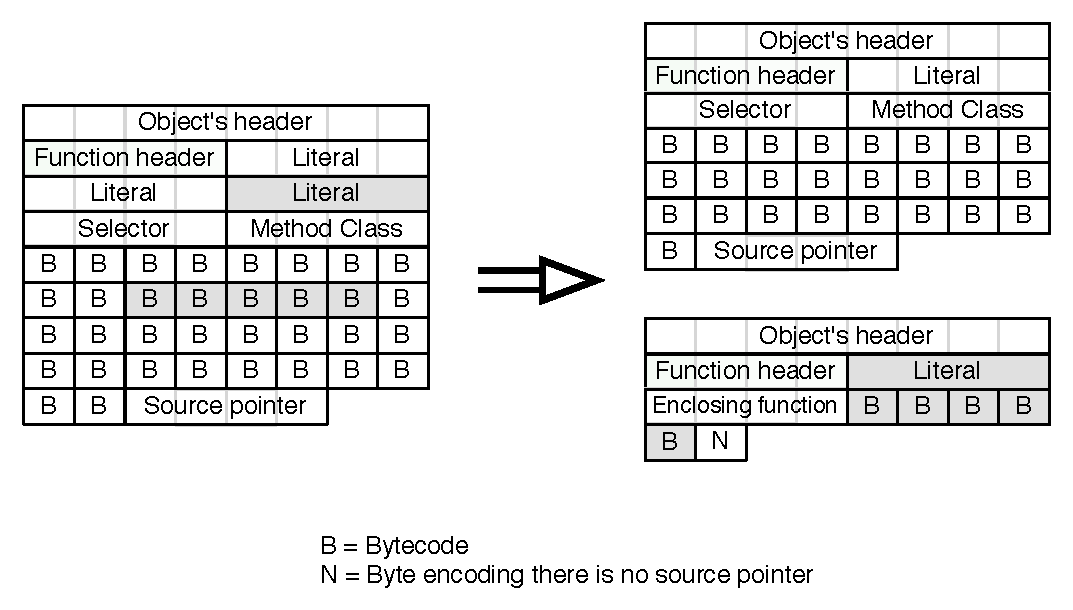
\includegraphics[width=0.85\linewidth]{CompiledBlock}
        \caption{Old and new closure representation}
        \label{fig:CompiledBlock}
    \end{center}
\end{figure}

Figure \ref{fig:CompiledBlock} shows on the left the old closure function representation and on the right the new representation. In the old representation, the closure function literals and bytecodes are present inside the enclosing function. The creation of a closure in the v-function interpreter requires to jump over the closure instructions. All the function metadata, normally present in the function header, can be computed by disassembling the closure creation instruction or the closure bytecodes. Any change on the closure function impacts the enclosing function and any change on the enclosing function impacts the closure function. When Cogit compiles the v-function to n-function, it compiles both the function and all the inner closure functions at the same time. In the new representation, the two functions are independent. Each function has its own function header. Both functions can be changed independently. Cogit compiles separatedly each v-function to n-function. The closure function has no source pointer as it can be fetched from the enclosing function.


\ifx\wholebook\relax\else
    \end{document}
\fi